\documentclass[11pt,table]{beamer}
\usepackage{verbatim} % For using /begin{comment}; /end{comment}
\setbeamertemplate{footline}{%
    \raisebox{5pt}{\makebox[\paperwidth]{\hfill\makebox[10pt]{%
    \scriptsize\insertframenumber}}}}
\setbeamertemplate{navigation symbols}{}% Empty to get rid of them!
\setbeamertemplate{itemize items}{$\circ$}
\usepackage{multirow}
\usepackage{booktabs}
\usepackage{textpos}
\usepackage{graphicx}
%\useoutertheme{infolines}
%\graphicspath{{images/}}
%\setbeamerfont{frametitle}{series=\bfseries} % Frame titles should be bold
\usepackage{lmodern}

\addtobeamertemplate{block begin}{\vspace{-8pt}}{}

\definecolor{flilac}{rgb}{0.53, 0.38, 0.56}
\definecolor{amethyst}{rgb}{0.6, 0.4, 0.8}
\definecolor{lightgrey}{rgb}{0.75, 0.75, 0.80}
\definecolor{tangerine}{rgb}{1.0, 0.6, 0.4}
\definecolor{arylyellow}{rgb}{0.91, 0.84, 0.42}
\definecolor{gsa}{rgb}{0.66, 0.89, 0.63}
\definecolor{aqua}{rgb}{0.5, 1.0, 0.83}
\definecolor{bblue}{rgb}{0, 0.72, 0.92}
\definecolor{cblue}{rgb}{0.53, 0.81, 0.98}

\definecolor{bittersweet}{rgb}{1.0, 0.44, 0.37}

\setbeamercolor{background canvas}{bg=black}
\setbeamercolor{normal text}{fg=white}
\setbeamercolor{title}{fg=arylyellow}
\setbeamercolor{frametitle}{fg=tangerine}
\setbeamercolor{framesubtitle}{fg=gsa}
\setbeamercolor{block title}{fg=cblue}
\setbeamercolor{itemize item}{fg=gsa} % all frames will have red bullets
\setbeamercolor{itemize subitem}{fg=tangerine} % all frames will have red bullets
\setbeamercolor{enumerate item}{fg=gsa} % all frames will have red bullets
\setbeamercolor{enumerate subitem}{fg=tangerine} % all frames will have red bullets

\newcommand\Wider[2][3em]{%
    \makebox[\linewidth][c]{%
       \begin{minipage}{\dimexpr\textwidth+#1\relax}
           \raggedright#2
       \end{minipage}%
    }%
}

\title{\textbf{Coronal Seismology}}
\subtitle{\textbf{ASTR 598}}
\date{\textbf{Spring 2016}}
\author{\textbf{Laurel Farris}}

\begin{document}
{\usebackgroundtemplate{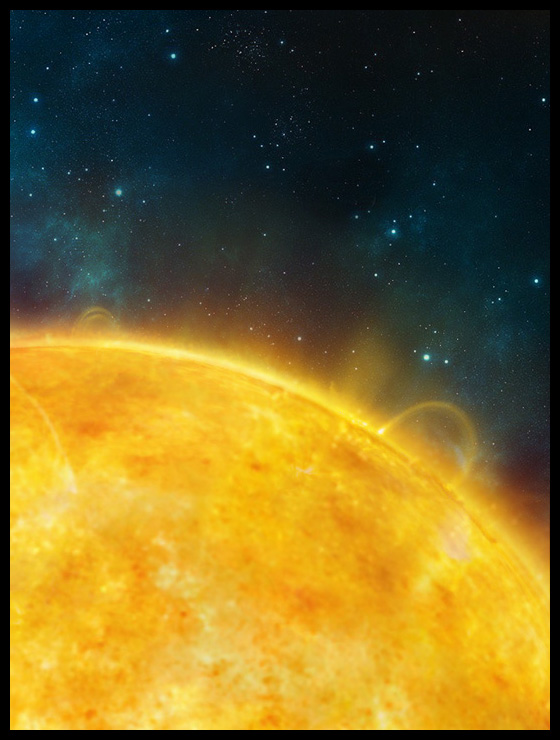
\includegraphics[width=\paperwidth]
    {awesome.jpg}}
\begin{frame}
    \titlepage{}
\end{frame}}%-------------------------------------------------------------%
\begin{frame}{Magnetohydrodynamics (MHD)}{Theory}
    \begin{columns}
        \column{0.45\textwidth}
        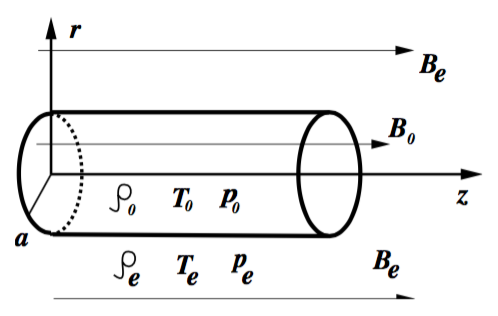
\includegraphics[width=\textwidth]{cylinder.png}\\
        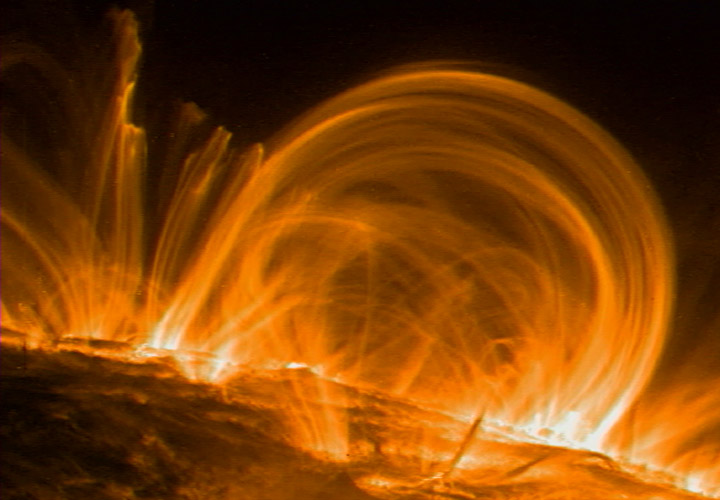
\includegraphics[width=\textwidth]{loop.jpg}
        \column{0.55\textwidth}
        \begin{block}{Model}
            \begin{itemize}
                \item Straight cylindrical flux tube in uniform magnetic field.
                \item $ \xi(x) = \xi(r)e^{i(kz+m{\phi})} $
                \item Characteristic wave speeds are determined by
                    $\rho$, $T$, $P$, and $\vec{B}$
            \end{itemize}
        \end{block}
        \begin{block}{Sound speed}
            \begin{itemize}
                \item $C_s \propto \sqrt{\cfrac{P}{\rho}} \propto \sqrt{T}$
            \end{itemize}
        \end{block}
        \begin{block}{Alfv\'en speed}
            \begin{itemize}
                \item $V_A \propto \cfrac{B}{\sqrt{\rho}}$
            \end{itemize}
        \end{block}
    \end{columns}
\end{frame}%-------------------------------------------------------------%
\begin{frame}{MHD modes}{Research Topics}
    \begin{columns}
        \column{0.5\textwidth}
        \begin{enumerate}
            \item Kink oscillations
            \item Sausage oscillations
            \item Acoustic oscillations
            \item Propagating acoustic waves
            \item Propagating fast waves
            \item Torsional (Alfv\'en) modes
        \end{enumerate}
        \begin{itemize}
            \item Magnetoacoustic
                %$C_s = \sqrt{\frac{\gamma P}{\rho}}$
                \begin{itemize}
                    \item Fast %$k_{A_0} < C_{fast} < C_{A_e} $
                    \item Slow %$C_{T_0} < C_{slow} < C_{s_0} $
                \end{itemize}
            \item Alfv\'en
                %$V_A = \frac{B}{\sqrt{\mu_0\rho}}$
        \end{itemize}
        \column{0.5\textwidth}
        \begin{block}{\centering Dispersion diagram}
        \begin{figure}
            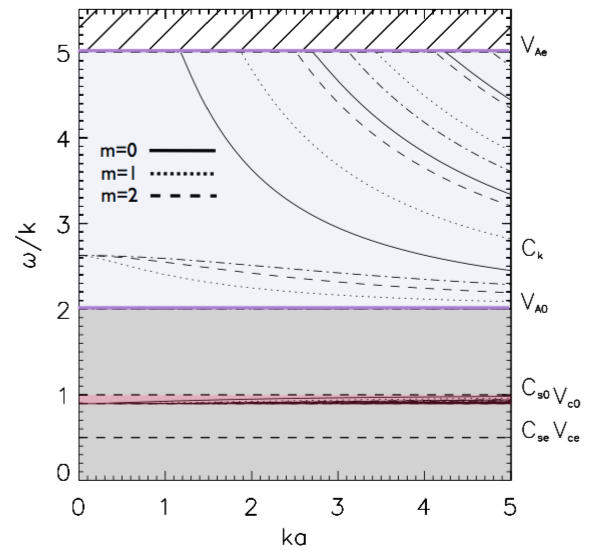
\includegraphics[width=\textwidth]{disp_diagram.png}
        \end{figure}
        $$ C_k = \sqrt{\frac{2}{1+\rho_e/\rho_o}}  $$
    \end{block}
    \end{columns}
\end{frame}%-------------------------------------------------------------%
\begin{frame}{Coronal seismology}{Technique and motivation}
    \begin{columns}
        %\column{0.5\paperwidth}
        \column{0.5\textwidth}
        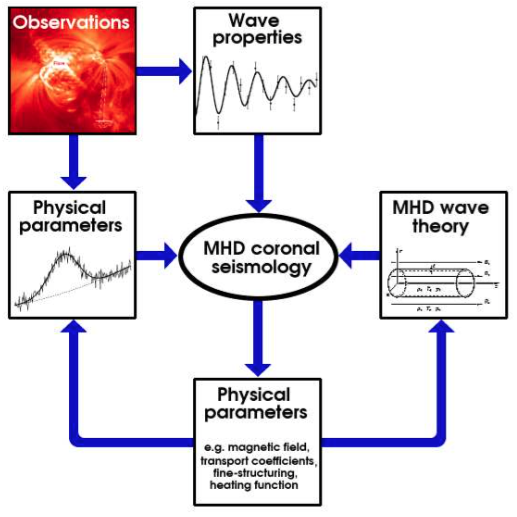
\includegraphics[width=\textwidth]{schematic.png}
        %\column{0.5\paperwidth}
        \column{0.5\textwidth}
        \begin{block}{Elusive coronal properties}
            \begin{itemize}
                \item magnetic field strength, $\vec{B}$
                \item density, $\rho$
                \item Alfv\'en velocity, $V_A$
            \end{itemize}
        \end{block}
        \begin{block}{Motivation}
            \begin{itemize}
                \item Coronal heating
                \item Space weather prediction
            \end{itemize}
        \end{block}
        \begin{block}{Coronal seismology}
            \begin{enumerate}
                \item Observe disturbances
                \item Measure properties
                \item Identify the wave or mode
                \item Extract coronal parameters
            \end{enumerate}
        \end{block}
    \end{columns}
\end{frame}%-------------------------------------------------------------%
\begin{frame}{Fast standing oscillations}{Kinks vs.\ Sausages}
    \begin{columns}
        \column{0.5\textwidth}
        %\begin{center}
            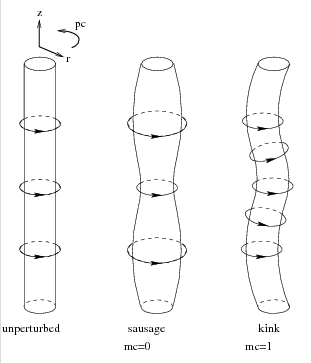
\includegraphics[width=\textwidth]{kink_saus.png}
        %\end{center}
        \column{0.5\paperwidth}
        \vspace{-0.5in}
        \begin{block}{Period}
            \begin{itemize}
                \item $P=\frac{2\ell}{V_{ph}}$
                    ($\lambda=2\ell$)
            \end{itemize}
        \end{block}
        \begin{block}{Kink}
            \begin{itemize}
                \item loop spatial displacement
                \item Asymmetric
                \item No intensity change
            \end{itemize}
        \end{block}
        \begin{block}{Sausage}
            \begin{itemize}
                \item No loop spatial displacement
                \item Symmetric
                \item Intensity change\\ $\rightarrow$ density change
            \end{itemize}
        \end{block}
\end{columns}
\end{frame}%-------------------------------------------------------------%

\begin{comment}
\begin{frame}{Standing oscillations vs.\ propagating waves}
    \begin{itemize}
        \item In loops, propagating waves damp before
            reaching opposite footpoint.
        \item Velocity and intensity are 90$^{\circ}$ out of phase
            for standing oscillations, and are in phase for propagating
            acoustic waves.
        \item Frequencies less than the cutoff are standing oscillations,
            waves with frequency greater than the cutoff propagate into
            the chromosphere.
    \end{itemize}
\end{frame}%-------------------------------------------------------------%
\begin{frame}{Torsional modes}{(Alfv\'en waves)}
    \begin{columns}
        \column{0.5\textwidth}
        \begin{block}{Properties}
            \begin{itemize}
                \item transverse (shear) perturbations
                \item Parallel to $\vec{B}$
                \item Driving force: magnetic tension
                \item incompressible (no twisting)
                \item $v_{A} = \frac{B}{\mu_{o}\rho} \approx 1000$
                    km s$^{-1}$
            \end{itemize}
        \end{block}
        \begin{block}{How to observe}
            \begin{itemize}
                \item Doppler shifts from \emph{long}-period waves
                    ($>$ a few minutes) reveal spatial variation;
                    Gyrosynchrotron emission in radio regime.
                \item non-thermal broadening
                    of coronal emission lines;
                    indirect way to observe short-period waves.
            \end{itemize}
        \end{block}
        \begin{block}{Effects of twisting}
            \begin{itemize}
                \item Coupling of various MHD modes
            \end{itemize}
        \end{block}
        \column{0.5\textwidth}
    \end{columns}
\end{frame}%-------------------------------------------------------------%
\end{comment}
\begin{frame}{Coronal loop oscillations observed with \emph{TRACE}}
    {Aschwanden et al. 1999}
    \begin{columns}
        \column{0.5\textwidth}
        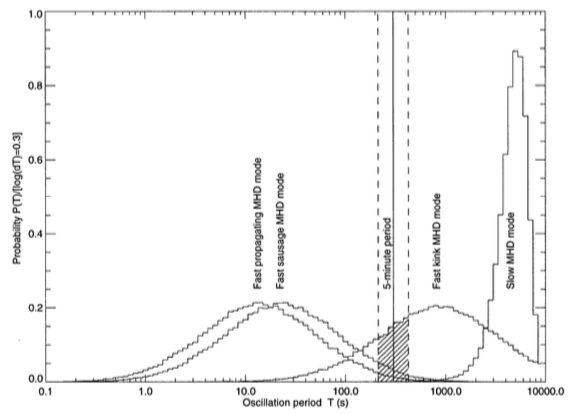
\includegraphics[width=\textwidth]{kink7.png}
        \column{0.5\textwidth}
    \end{columns}
\end{frame}%-------------------------------------------------------------%
\begin{frame}
    \vspace{0.25cm}
    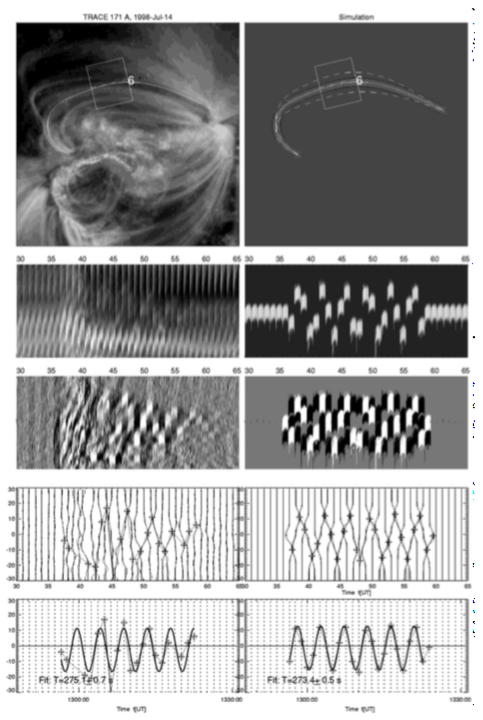
\includegraphics[height=\textheight]{kink3.png}
\end{frame}%-------------------------------------------------------------%
\begin{frame}{Excitation and damping of broadband kink waves in the solar
    corona}
\end{frame}%-------------------------------------------------------------%
\begin{frame}[t]{``Observations of sausage modes in magnetic pores''}
    {Morton et al. 2011}
    \begin{block}{}
        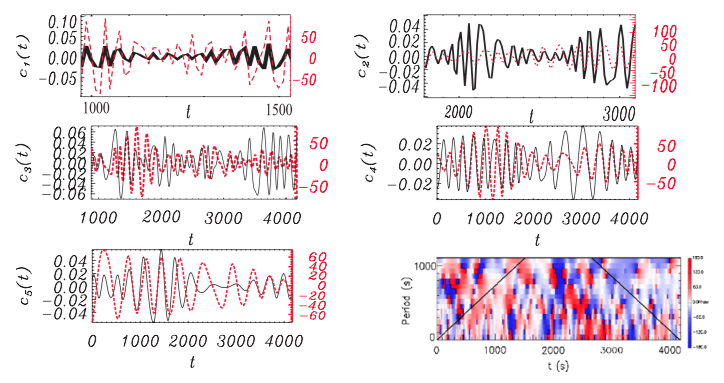
\includegraphics[width=\textwidth]{saus2.png}
    \end{block}
    \begin{block}{}
        \begin{itemize}
            \item Periods $\sim$ 30--450 sec
            \item Possibly driven by 5-min acoustic oscillations.
        \end{itemize}
    \end{block}
\end{frame}%-------------------------------------------------------------%
\begin{frame}[t]{Acoustic waves}{A. K. Srivastava and B. N. Dwivedi}
    \begin{columns}
        \column{0.5\textwidth}
            %\item Parallel to $\vec{B}$, perturbation of $\vec{B}$ is negligible.
            %\item Generated impulsively at one end of a footpoint.
            %\item Only penetrate $\sim$ 10\% into loop before
            %    damped by thermal conduction
            %\item weak dispersion in coronal conditions ($V_{A} \gg c_{s}$)
            %\item 3 phases: periodic, QP, decay
            %\item period = 3, 5, 10 minutes? Or 2--22 seconds? (see kink\_1),
            %\item velocity: 50--200 km s$^{-1}$
            %\item $c_{T} = \sqrt{\frac{c_{s}^2v_{A}^2}{c_{s}^2 + v_{A}^2}} $
            %    propagate sub-sonically at $c_{T}$, which is less than $c_{s}$
            %\item Observed using spectroscopy (intensity variations in
            %    EUV emission  and Doppler shifts)
        \begin{block}{Observed}
            \begin{itemize}
                \item Time series of a bright point (BP) in solar atmosphere
            %with EIS on \emph{HINODE}
            \end{itemize}
        \end{block}
        \begin{block}{Measured Periods}
            \begin{itemize}
                \item He {\footnotesize II} 256 \AA{}; P$\sim$ 263 s
                \item Fe {\footnotesize XII} 195 \AA{}
                \item Fe {\footnotesize XV} 284 \AA{}; P$\sim$ 241 s
            \end{itemize}
        \end{block}
        \begin{block}{Identified}
            \begin{itemize}
                \item Acoustic oscillations leaking into the inner corona
            \end{itemize}
        \end{block}
        \column{0.6\textwidth}
        \begin{block}{}
            \vspace{-0.5in}
            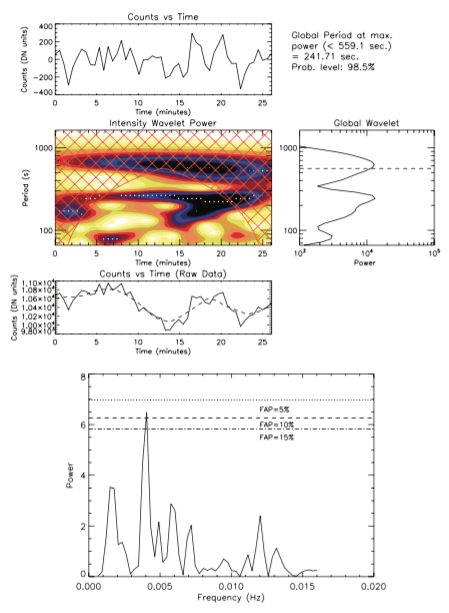
\includegraphics[height=0.9\paperheight]{ex1.png}
        \end{block}
    \end{columns}
\end{frame}%-------------------------------------------------------------%
\begin{frame}{Alfv\'en waves}{Verwichte et al.}
    \begin{columns}
        \column{0.5\textwidth}
        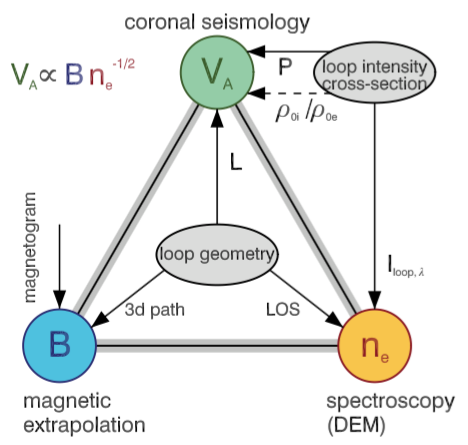
\includegraphics[width=\textwidth]{tor2.png}
        \column{0.5\textwidth}
        \begin{block}{Objective}
            \begin{itemize}
                \item Determine Alfv\'en speed in two ways:
                    \begin{enumerate}
                        \item Coronal seismology
                        \item Magnetic extrapolation and spectral methods
                    \end{enumerate}
            \end{itemize}
        \end{block}
        \begin{block}{Observed}
            \begin{itemize}
                \item Two transversely oscillating flares triggered by flare
                \item AIA/SDO 171 \AA{}
            \end{itemize}
        \end{block}
    \end{columns}
\end{frame}%-------------------------------------------------------------%


\begin{comment}
\begin{frame}[t]{Slow magnetoacoustic waves}{Robbrecht, et al. (2001)}
    \begin{block}{}
        %\column{0.5\textwidth}
        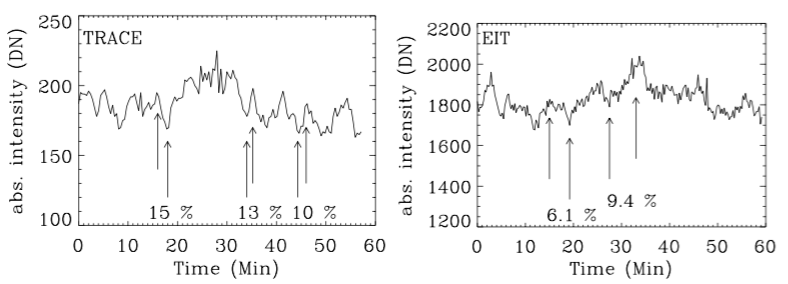
\includegraphics[width=\textwidth]{pac1.png}
        %\column{0.5\textwidth}
    \end{block}
    \begin{block}{}
        \begin{itemize}
            \item Multi-wavelength observations
            \item Same wave, different speeds at different temperatures
            \item Loop contains sharp temperature gradient
        \end{itemize}
    \end{block}
\end{frame}%-------------------------------------------------------------%
\end{comment}


\begin{frame}{Important Properties}{From papers, reviews, etc.}
\begin{center}
    \begin{tabular}{c|c|c|c|}
        \cline{2-4} & {\textbf{\textcolor{gsa}{period}}} &
        {\textbf{\textcolor{gsa}{decay time}}} &
        {\textbf{\textcolor{gsa}{velocity}}}\\
        \hline \multicolumn{0}{|c|}{\textcolor{bblue}{kink osc}} &
            2{-}20 m & quickly & value\\
        \hline \multicolumn{0}{|c|}{\textcolor{bblue}{sausage osc}} &
            30 s{-}7 m & value & value\\
        \hline \multicolumn{0}{|c|}{\textcolor{bblue}{acoustic osc}} &
            7{-}31 m & 5{-}30 m & 200 km s$^{-1}$\\
        \hline \multicolumn{0}{|c|}{\textcolor{bblue}{acoustic waves}} &
            value & value & $<$150 km s$^{-1}$\\
        \hline \multicolumn{0}{|c|}{\textcolor{bblue}{fast waves}} &
            value & value & $>$150 km s$^{-1}$\\
        \hline \multicolumn{0}{|c|}{\textcolor{bblue}{torsional modes}} &
            10 m & long & 1000 km s$^{-1}$\\
        \hline
    \end{tabular}
\end{center}
\end{frame}%-------------------------------------------------------------%
{%
\setbeamercolor{background canvas}{bg=black}
\setbeamertemplate{background}{%
\parbox[c][\paperheight][c]{\paperwidth}{%
%\hspace{3cm}
\centering
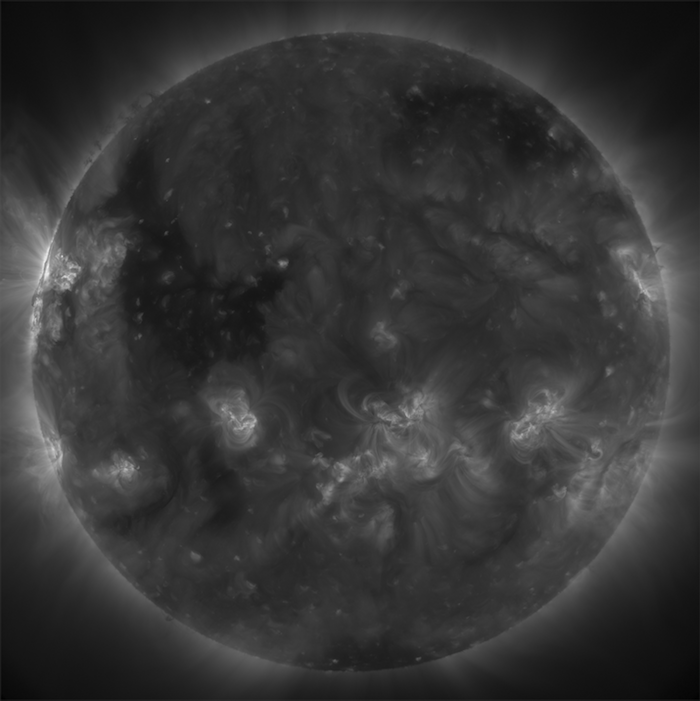
\includegraphics[height=\paperheight]{figures/full_disk.png}}}
\begin{frame}[t]{Research}{AIA/SDO}
    \hspace{-2em}Fe {\footnotesize XII, XXIV}\\
    \hspace{-2em}193 \AA{}\\
\end{frame}}%------------------------------------------------------------%
\begin{comment}
\begin{frame}[c]{Research}{[Looks nicer than white background]}
    \includegraphics[width=0.7\paperwidth]{figures/bp1.png}
\end{frame}%-------------------------------------------------------------%
\begin{frame}[c]{Research}
    \includegraphics[width=0.8\paperwidth]{figures/bp1_image.png}
\end{frame}%-------------------------------------------------------------%
\end{comment}%===========================================================%
\begin{frame}{Research}{Bright point (BP)}
    \centering
    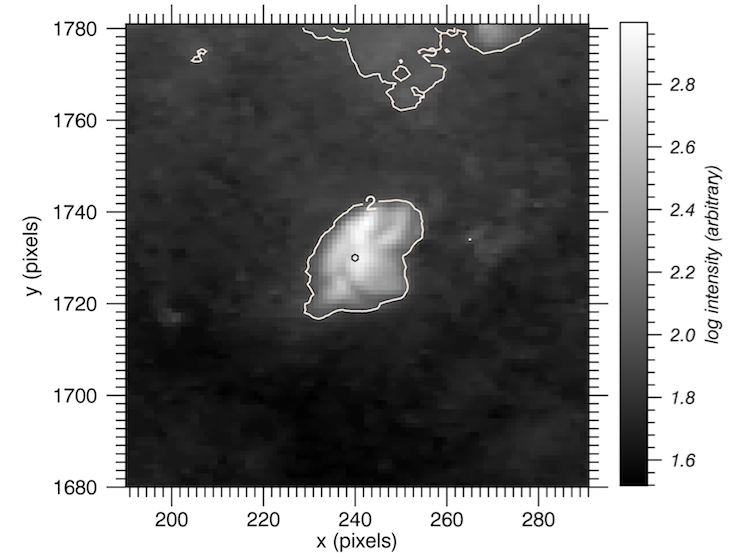
\includegraphics[width=0.7\paperwidth]{figures/bp1_contour.png}
\end{frame}%-------------------------------------------------------------%
\begin{frame}{Research}{Light curves}
    \begin{center}
        \includegraphics[width=0.8\paperwidth]{figures/lightcurve3.png}
    \end{center}
\end{frame}%-------------------------------------------------------------%
\begin{frame}{Research}{Cross-correlations}
    \begin{block}{}
        \begin{columns}
            \column{0.3\textwidth}
            \includegraphics[width=0.2\paperwidth]{figures/bp1.png}
            \column{0.7\textwidth}
            \vspace{-2em}
            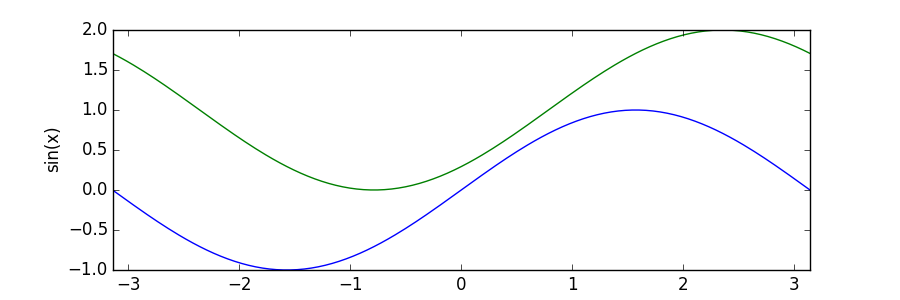
\includegraphics[width=\textwidth]{cross.png}
            %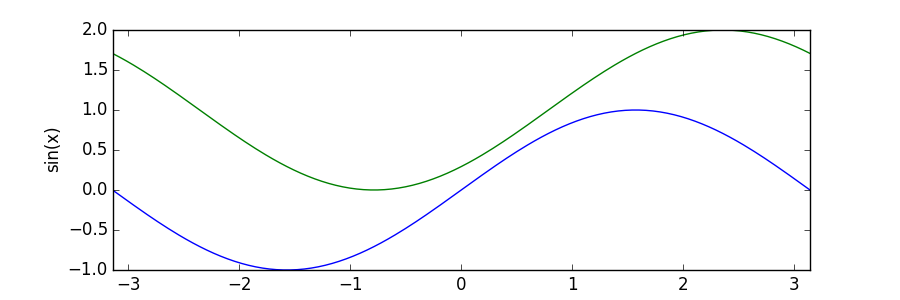
\includegraphics[keepaspectratio=false,width=0.9\textwidth,height=1in]{cross.png}
        \end{columns}
    \end{block}
    \begin{block}{}
    \Wider[4em]{%
    \begin{center}
        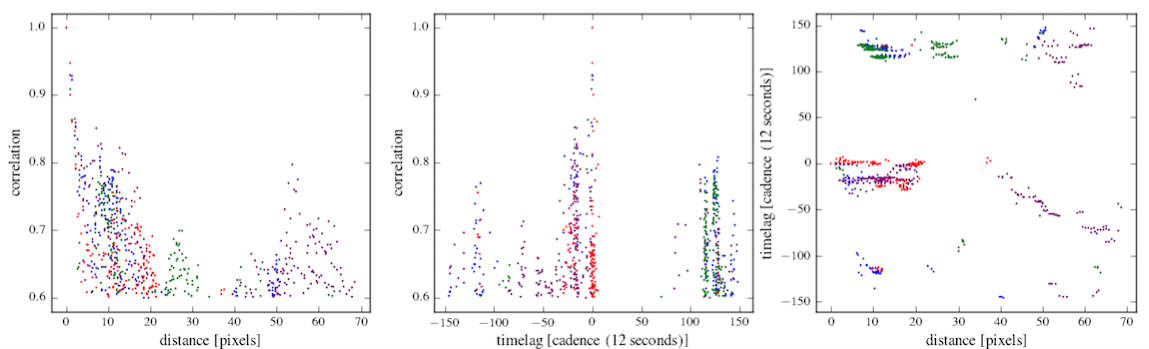
\includegraphics[width=\textwidth]{test2.png}
    \end{center}}
    \end{block}
\end{frame}%-------------------------------------------------------------%
\begin{frame}[t]{Research}{Cross-correlation \& timelag images}
\vspace{0.25in}
    \begin{columns}
        \column{0.5\textwidth}
        \begin{block}{\centering Cross-correlation}
            \begin{center}
                \vspace{-0.25in}
                \includegraphics[height=0.5\textheight]{figures/bp1_cc.png}
            \end{center}
        \end{block}
        \column{0.5\textwidth}
        \begin{block}{\centering Timelag}
            \begin{center}
                \vspace{-0.25in}
                \includegraphics[height=0.5\textheight]{figures/bp1_tt2.png}
            \end{center}
        \end{block}
    \end{columns}
    \begin{center}
        2 pixels $\sim$ 1 arcsec $\sim$ 700 km
    \end{center}
\end{frame}%-------------------------------------------------------------%
\begin{frame}{Other questions and future work}
    \begin{block}{Other questions}
        \begin{itemize}
            \item What is the excitation mechanism for the observed
                disturbances?
            \item How are they damped, and what determines the timescales?
        \end{itemize}
    \end{block}
    \begin{block}{My future work}
        \begin{itemize}
            \item Download data in other wavelengths (i.e.\ coronal heights).
            \item Download data from other instruments,
                e.g.\ the Extreme Ultraviolet Variability Experiment
                (EVE) on SDO\@.
            \item Characterize other bright points in coronal hole,
                quiet sun, and active regions.
        \end{itemize}
    \end{block}
\end{frame}%-------------------------------------------------------------%
\begin{frame}{Acknowledgements}
    Advisor: James McAteer
\end{frame}%-------------------------------------------------------------%

\begin{frame}{Extra slides here}
\end{frame}

\end{document}
